\documentclass[11pt,a4paper]{ivoa}
\input tthdefs

\newcommand{\xtype}[1]{\texttt{#1}}
\newcommand{\ucd}[1]{\texttt{#1}}

\usepackage{listings}
\lstloadlanguages{XML,sh}
\lstset{flexiblecolumns=true,basicstyle=\small,tagstyle=\ttfamily}
\usepackage[utf8]{inputenc}
\usepackage{todonotes}

\title{IVOA Architecture}

\ivoagroup{Technical Coordination Group}

\author{Patrick Dowler}
\author{Janet Evans}
\author{etc}
\author{etc}
\author{etc}

\editor{Patrick Dowler, Janet Evans}

\previousversion{IVOAArchitecture-1.0-20101123}

\begin{document}

\begin{abstract}
This note describes the technical architecture of the IVOA. The description is decomposed into three levels. Level 0 is a general, high level summary of the IVOA Architecture. Level 1 provides more details about components and functionalities, still without being overly technical. Finally, Level 2 displays how the IVOA standards fit into the IVOA Architecture. 
\end{abstract}

\section*{Acknowledgments}

\section{IVOA Architecture Level 0}

\begin{figure}
\centering
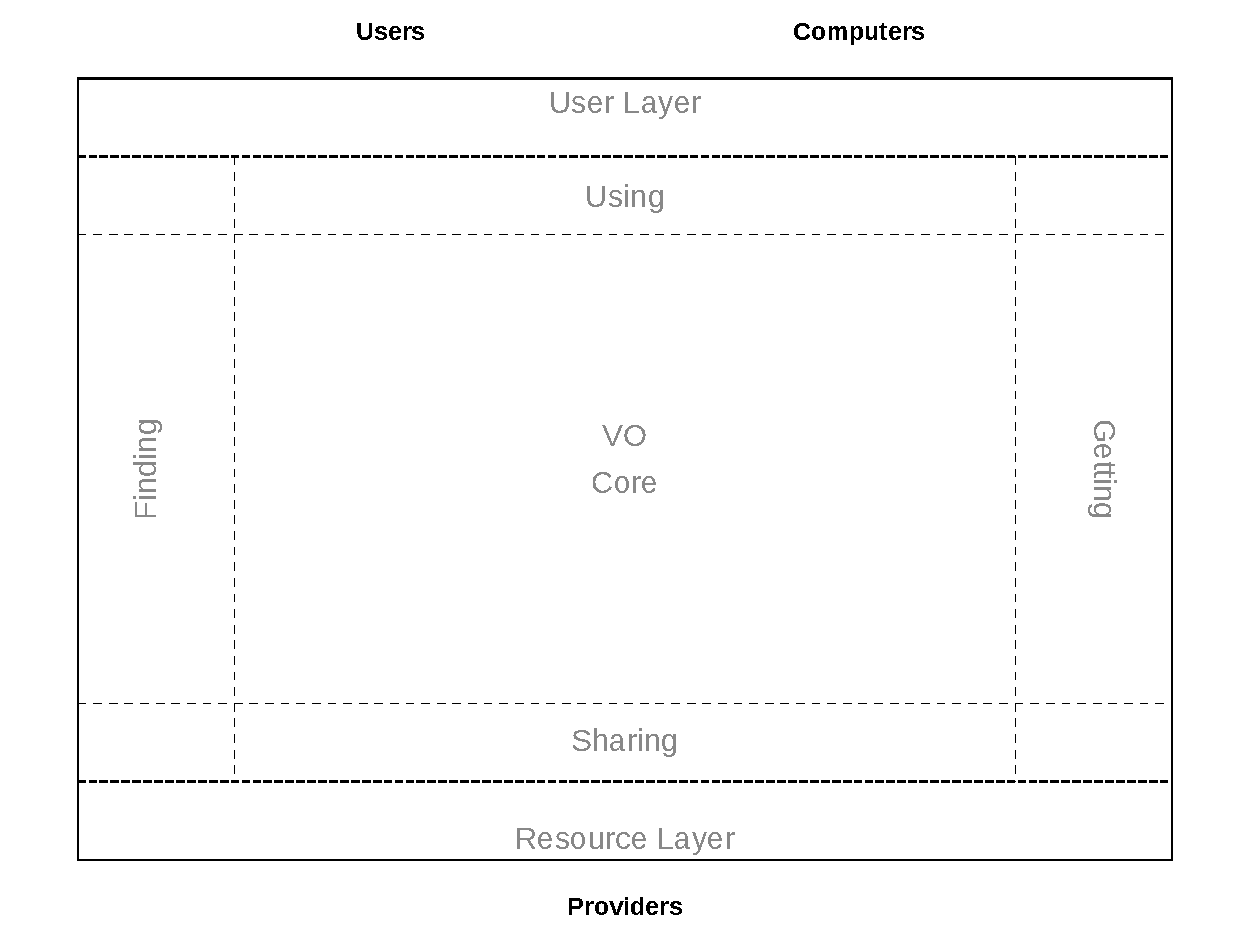
\includegraphics[width=0.9\textwidth]{archdiag0.png}
\caption{IVOA Architecture Level 0}
\label{fig:architecture}
\end{figure}

Astronomy produces large amounts of data of many kinds, coming from various sources: science  space missions, ground based telescopes, theoretical models, compilation of results, etc.  These data are usually managed by large data centres or smaller teams. These providers provide  the scientific community with data and/or computing services through the Internet. This is the Resource Layer. 

The ``consumer'' of these data and computing services, be it individual researchers, research teams or computer systems, interact with the User Layer. 

The Virtual Observatory is the necessary ``middle layer'' framework connecting the Resource Layer to the User Layer in a seamless and transparent manner. Like the web which enables end  users and machines to access transparently documents and services wherever and however they are stored, the VO enables the astronomical scientific community to access astronomical resources   wherever and however they are stored by the astronomical data and services providers. The VO provides a technical framework for the providers to share their data and services (``Sharing''), and allowing users to find (``Finding'') these resources, to get them (``Getting'') and to use them (``Using''). To enable these functionalities, the definition of some core astronomically-oriented standards (``VO Cor'') is also necessary.

\section{IVOA Architecture Level 1}

Level 1 of the IVOA architecture is an extension to the Level 0, displaying more details about the functionalities and building blocks within the different layers. For completeness,  part  of  the  description  is  repeated  from  the  Level  0  one,  so  the  Level 1 description can be used as a self-contained block.

\begin{figure}
\centering
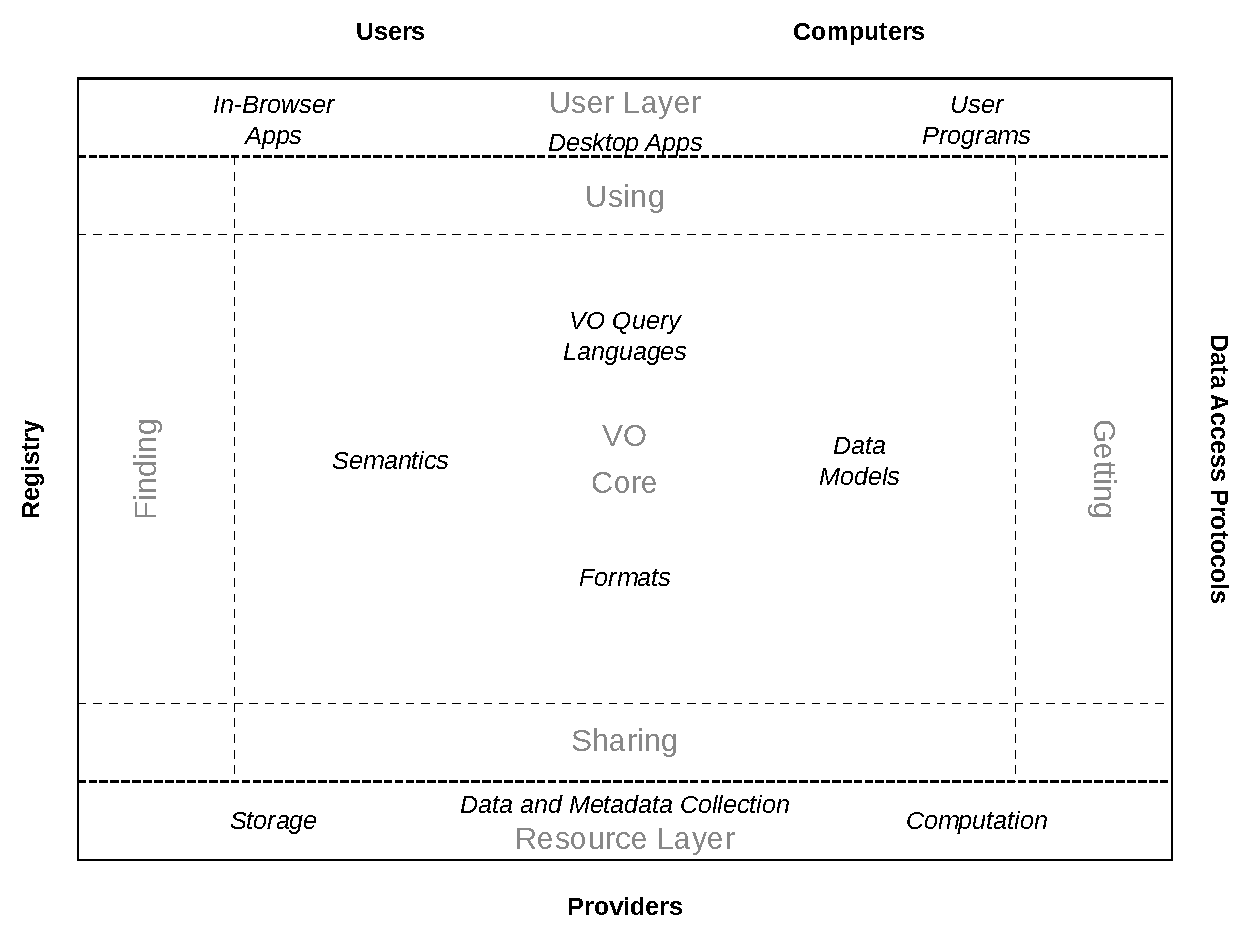
\includegraphics[width=0.9\textwidth]{archdiag1.png}
\caption{IVOA Architecture Level 0}
\label{fig:architecture}
\end{figure}

TODO: user layer now contains: browser applications, desktop applications, script applications, web portals, and platforms

\section{IVOA Architecture Level 2}

Level 2 of the IVOA Architecture is similar to the Level 1, but adds all the IVOA standards in  their corresponding layer.

\begin{figure}
\centering
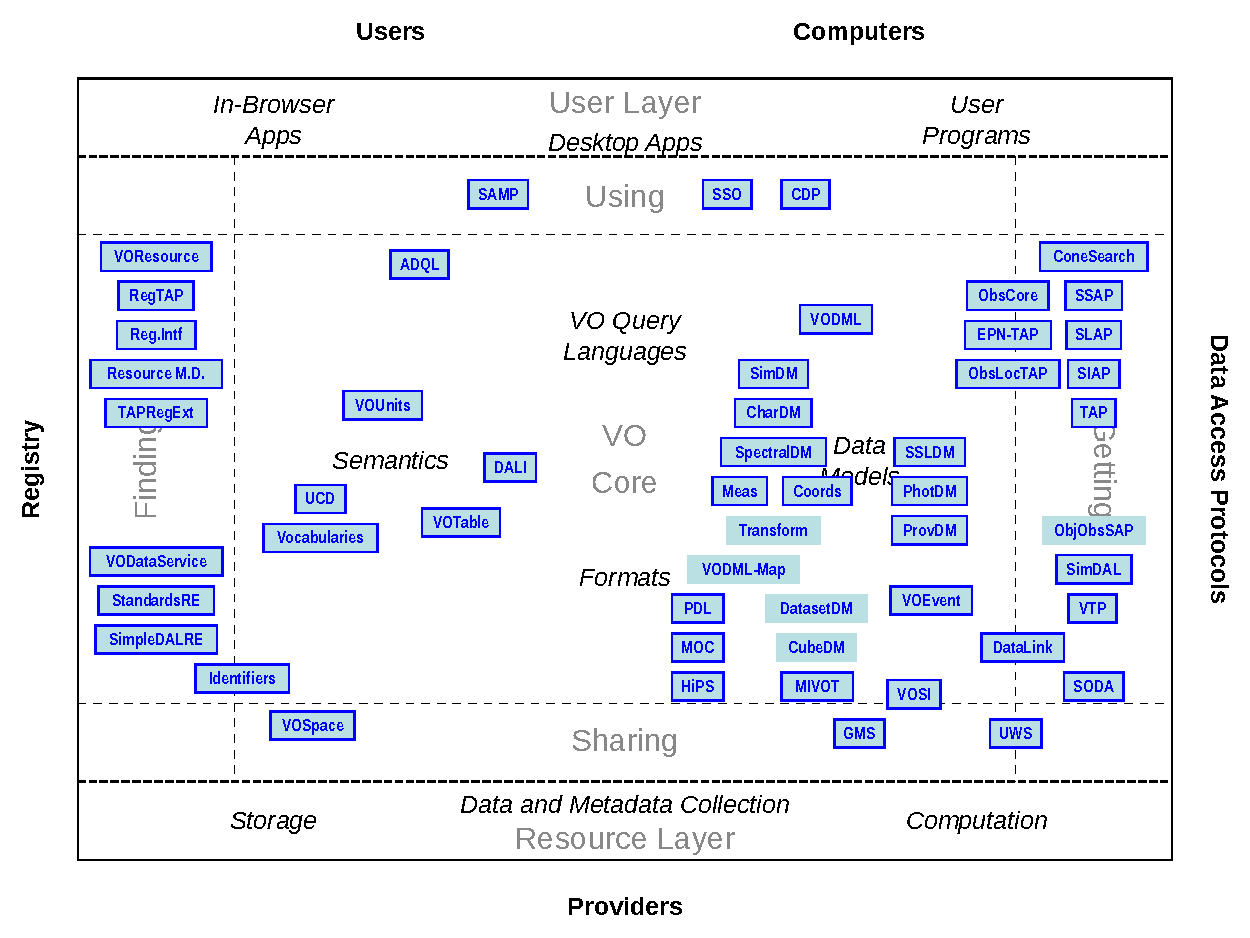
\includegraphics[width=0.9\textwidth]{archdiag2.png}
\caption{IVOA Architecture Level 0}
\label{fig:architecture}
\end{figure}

Some  standards  have  already  been  approved and recommended (blue boxes with an outer line) while others are still being worked on (blue boxes without an outer line). Note that this list  (and standard  status) will naturally evolve with time. More standards will be approved and recommended. Additionally, as driven by science use cases, new standards will be identified and added to that Figure X. The following sections provide a summary description of each individual standard, including where it fits into the IVOA architecture and its possible links with other IVOA standards.

\section{Finding: Registry Standards}

\section{Getting: Data Access Standards}

\section{Core: Data Model Standards}

\section{Core: Query Language Standards}

\section{Core: Semantics Standards}

\section{Core: Format Standards}

\section{Using: Application Standards}

\section{Sharing: Resource Access Standards}

\subsection{Changes from IVOAArchitecture-1.0-20101123}

TODO

\bibliography{ivoatex/ivoabib}

\end{document}
